%# -*- coding: utf-8 -*-
% automata.tex
% asymptotebyexample 的一章,流程图、结构体、运算符重载等内容

\chapter{严教授的自动机}

严宇教授是一位计算机语言专家。在他给学生讲授可计算性与自动机理论的课程时,需
要制做含有大量图论图形和自动机。一个典型的例子是描述正则语言的有限自动机,
\autoref{fig:automatahand} 就是严教授手绘的一个有限自动机。
\begin{figure}[htpb]
  \centering
  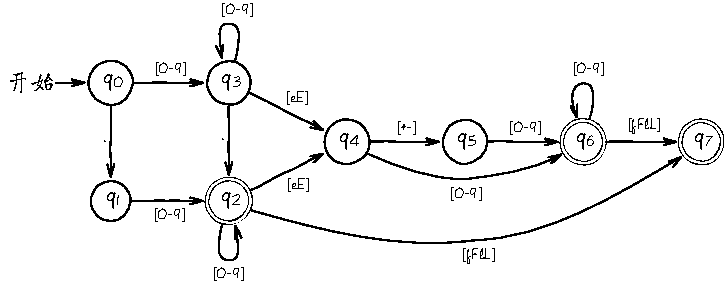
\includegraphics[scale=1.5]{automata_hand.pdf}
  \caption{严教授手画的有限自动机:它描述了 C 语言中浮点型字面值的词法。}
  \label{fig:automatahand}
\end{figure}

然而,尽管\autoref{fig:automatahand} 中严教授的自动机画得很仔细,但要在他的课
程幻灯片中使用,还是太粗疏了。严教授需要的是色彩鲜明、清晰准确的自动机图形,
就像\autoref{fig:automata} 中的一样。
\begin{figure}[htpb]
  \centering
  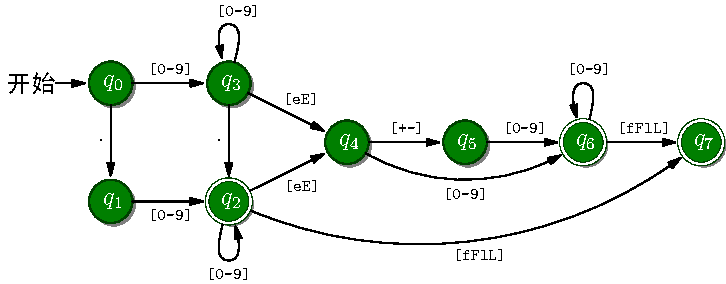
\includegraphics[scale=1.5]{automata.pdf}
  \caption{严教授想要在幻灯片里使用的有限自动机}
  \label{fig:automata}
\end{figure}

经过考虑,严教授决定用 \Asy{} 语言来完成这样的绘图,因为这样可以画出最精确的
图形,并能方便地对图形的所有细节进行控制,并且适合绘制大量形式相近的图形。然
而要让图形和生成图形的代码都接近完美,也将是一个艰巨的任务。

\section{标签和连线}

把一些相似的小图形用线和箭头连接起来,是应用中非常广泛的一种作图类型。工作程
序的流程图、电路设计图、网络结构图、计算机科学中的自动机、乃至古老的家谱,都
可以看作是这类图形。这些相似的小图形往往是以一个文字标签为中心、用某种形状的
曲线围成的,再以各种线连接为一个整体——它可以抽象为数学中的“图”。这类图形
可以统称为图论图形,这正是计算机科学中使用最多的一类图形,也是严宇教授工作的
重点。

\Asy{} 语言已经提供了一种给标签围上边框,再连上线条的方法。这依赖于一种特殊的
数据类型:|object|(物件)。一个物件就是一个带有某种形状边框的文字标签。函数
\begin{asycode}
object draw(picture pic=currentpicture, Label L, envelope e,
            pair position=(0,0), real xmargin=0, real ymargin=xmargin,
            pen p=currentpen, filltype filltype=NoFill);
\end{asycode}
将在图 |pic| 上的位置 |position| 画出一个以标签 |L| 为中心,边框形状为 |e| 的
物件。参数 |xmargin| 和 |ymargin| 是边框与标签边沿的距离,画笔 |p| 用来绘制文
字标签,而 |filltype| 控制边框如何绘制和填充。

\Asy{} 的这个函数初看起来非常复杂,但排除默认的参数,使用起来是直接了当的:
\begin{asycode}
object cat = draw("cat", box, (0,0), filltype=Draw),
       dog = draw("dog", ellipse, (2cm,0), filltype=Fill(olive)),
       elephant = draw("elephant", roundbox, (0,-2cm),
                       filltype=FillDraw(lightblue, darkblue));
\end{asycode}
\begin{figure}[H]
  \centering
\begin{asy}
object cat = draw("cat", box, (0,0), filltype=Draw),
       dog = draw("dog", ellipse, (2cm,0), filltype=Fill(olive)),
       elephant = draw("elephant", roundbox, (0,-2cm),
                       filltype=FillDraw(lightblue, darkblue));
\end{asy}
\end{figure}
这里 |box|、|ellipse| 和 |roundbox| 分别是矩形、椭圆和圆角矩形三种可以使用的
形状;|Draw|、|Fill|、|FillDraw| 则分别是对边框画线、填充的控制变量,如果不带
参数直接使用,默认是使用当前画笔(参考 \cite{asyman})。

\endinput

% vim:tw=77:

